\begin{frame}{Optimization}
    \begin{columns}
        \begin{column}{0.45\textwidth}
            \begin{itemize}
                \item To find the "best line," we should minimize the distances between our line’s predictions and all the data points.
                \item How to define that mathematically?
            \end{itemize}
        \end{column}
        \begin{column}{0.55\textwidth}
            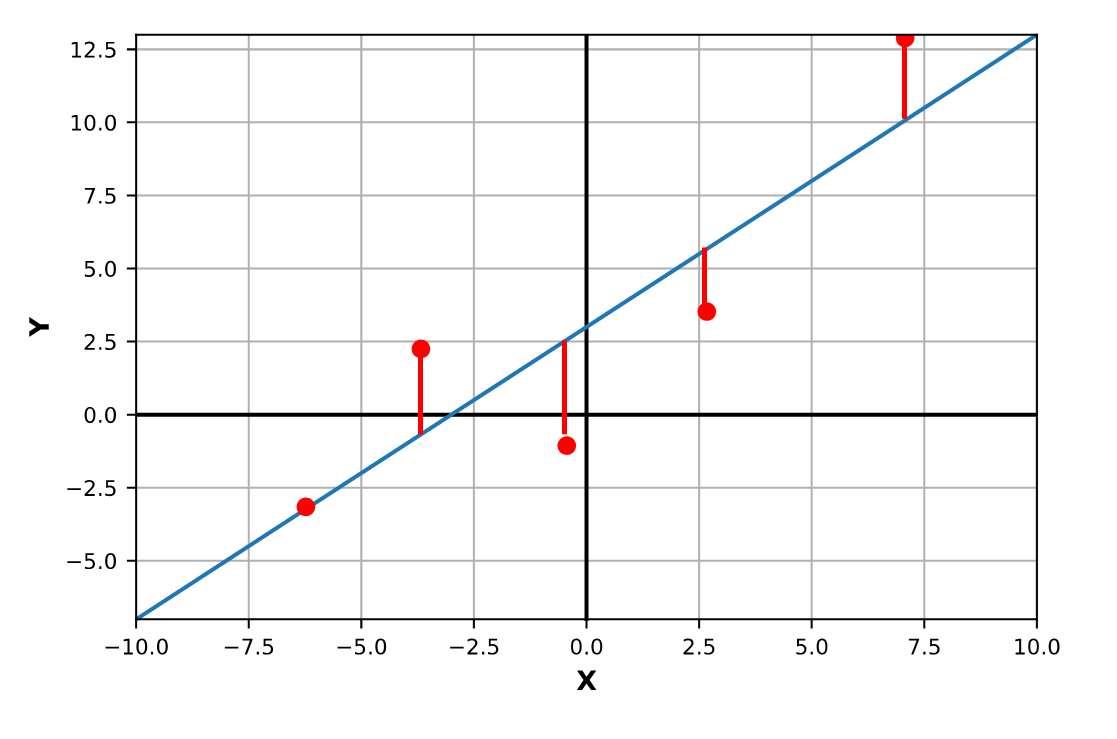
\includegraphics[width=\linewidth]{images/linear-regression/linear-regression-7.png}
        \end{column}
    \end{columns}
\end{frame}


\begin{frame}{Loss Function}
    \begin{itemize}
        \item For one sample, this can be represented mathematically by:
        \[
            (y_i - \hat{y}_i) \quad \text{(Error)}
        \]
        
        \item But this could result in negative value if $\hat{y} > y$. Let’s square it to remove the negative sign:
        \[
            (y_i - \hat{y}_i)^2 \quad \text{(Squared Error)}
        \]

        \item But we have $N$ samples, not only one. So, let’s sum the errors and take the average:
        \[
            \boxed{
                \text{Loss (MSE)} = \frac{1}{N} \sum_{i=1}^{N} (y_i - \hat{y}_i)^2
            }
            \quad \text{(Mean Squared Error)}
        \]
    \end{itemize}
\end{frame}


\begin{frame}{Cost Function Example}
    \begin{figure}
        \centering
        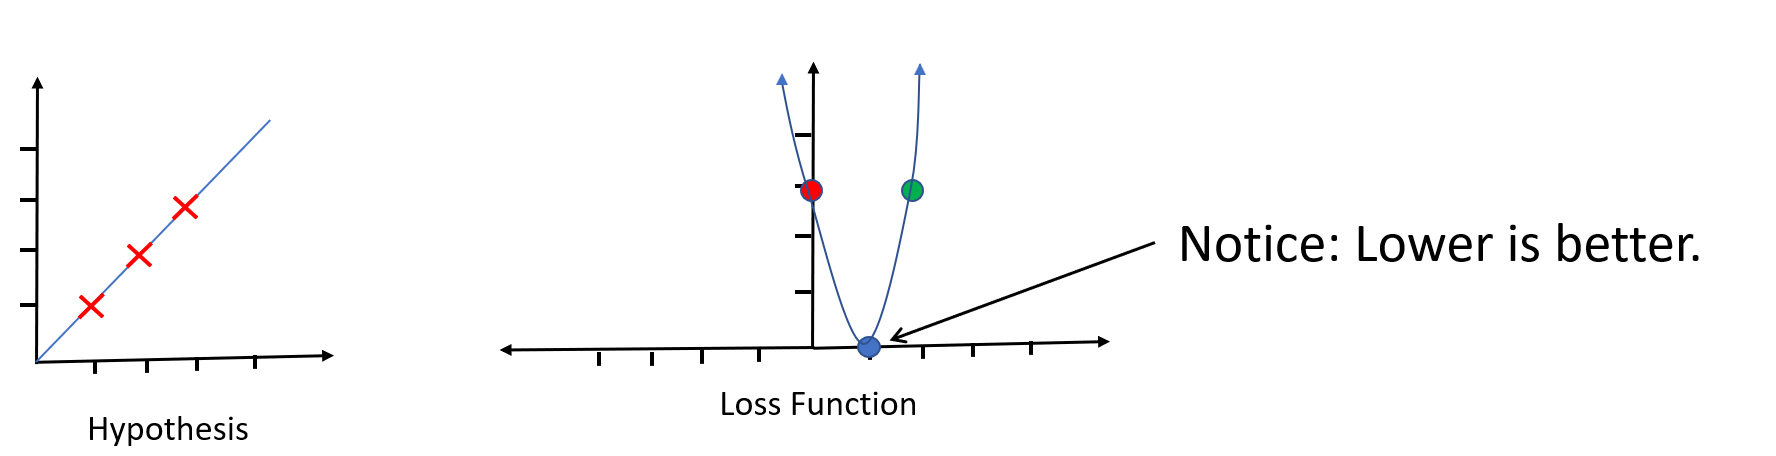
\includegraphics[width=0.9\textwidth]{images/linear-regression/linear-regression-8.png}
    \end{figure}

    \centering
    \fcolorbox{red}{white}{\strut\large $J(m=0) = 14$} \hspace{0.5cm}
    \fcolorbox{blue}{white}{\strut\large $J(m=1) = 0$} \hspace{0.5cm}
    \fcolorbox{green}{white}{\strut\large $J(m=2) = 14$}

    \[
        h(x) = mx \qquad
        J(m) = \sum_{i=1}^{3} (y_i - mx_i)^2
    \]
\end{frame}


\begin{frame}{How to find minima of a function (Review):}
    \begin{itemize}
        \item There are two approaches to find the minima:
        \begin{itemize}
            \item \textbf{Exact (Closed-form):} Directly calculates the solution mathematically by solving for $f'(x) = 0$.\\
            \underline{Important Note:} can be used only with a very limited number of algorithms.
            
            \item \textbf{Approximation (Iterative approach):} Gradually improves the solution step by step.\\
            Done by optimizers (e.g., Gradient Descent, ADAM, \ldots etc).
        \end{itemize}
    \end{itemize}
\end{frame}


\begin{frame}{How to find minima of a function (Review):}
    \centering
    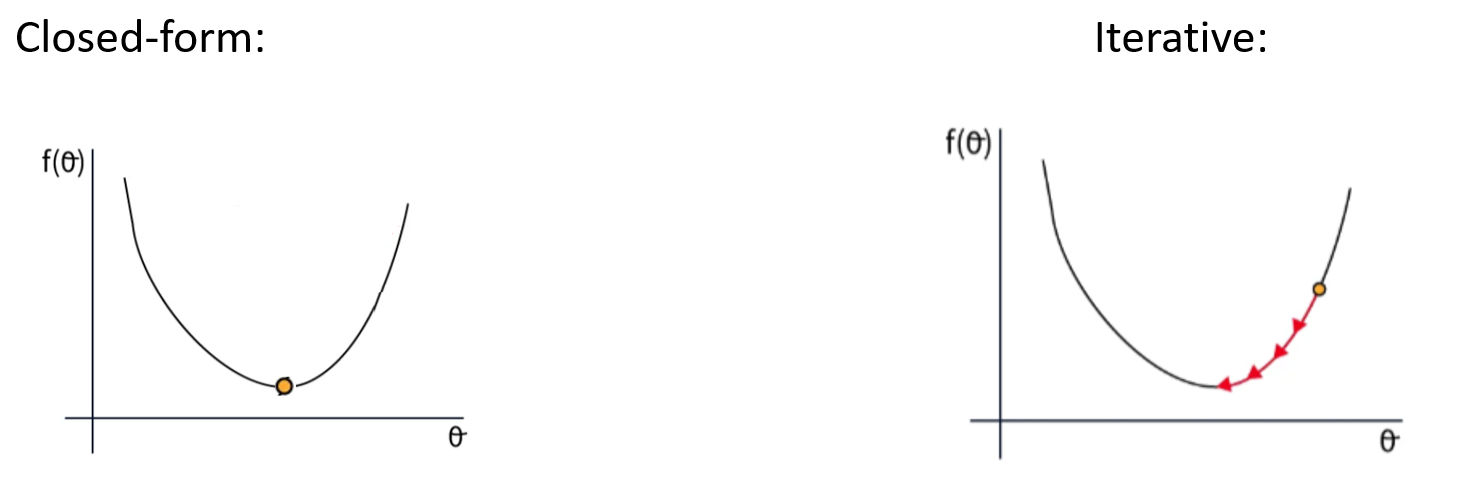
\includegraphics[width=0.8\linewidth]{images/linear-regression/linear-regression-9.png}

    \begin{itemize}
        \item \textbf{Example:} $y = x^2$ \quad (Solution: $x = 0$)
        \begin{itemize}
            \item Closed-form Final Result: $x = 0$
            \item Iterative Final Result: $x = 0.00001$ (close enough)
        \end{itemize}
    \end{itemize}
\end{frame}


\begin{frame}[allowframebreaks]{Review}

    \begin{center}
        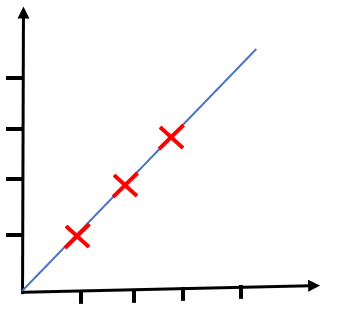
\includegraphics[width=0.7\linewidth]{images/linear-regression/linear-regression-10.png}

        \tiny \textit{(Notice that $y = x$ for our 3 points.)}
    \end{center}

\framebreak

    \begin{itemize}
        \item Let’s try to solve this using the closed-form here (Assume $\hat{y} = mx$):
    \end{itemize}

    \[
    J(m) = \sum_{i=1}^3 (y_i - mx_i)^2 
    \quad \Rightarrow \quad
    J(m) = \sum_{i=1}^3 (i - mi)^2
    \]

\framebreak

    \[
    \frac{dJ(m)}{dm} = \frac{d}{dm} \sum_{i=1}^3 (i - mi)^2
    \quad \Rightarrow \quad
    \frac{dJ(m)}{dm} = \sum_{i=1}^3 \frac{d}{dm}(i - mi)^2
    \]

\framebreak

    \[
    \frac{dJ(m)}{dm} = \sum_{i=1}^3 -2i(i - mi)
    \quad = \quad
    -2 \sum_{i=1}^3 i^2 + 2m \sum_{i=1}^3 i^2 
    \quad = \quad 0 
    \quad \Rightarrow \quad m = 1
    \]

\end{frame}


\begin{frame}{Hypothesis Function with 2 Variables}
    \begin{itemize}
        \item Let’s set up regression for a linear function in two variables:
        \item The hypothesis function is:
    \end{itemize}

    \begin{center}
        \[
        \hat{y}_i = mx_i + b
        \]
    \end{center}

    \begin{itemize}
        \item Similar to the previous problem, our loss function is:
    \end{itemize}

    \begin{center}
        \[
        J = \frac{1}{N} \sum_{i=1}^{N} (y_i - \hat{y}_i)^2
        \]
    \end{center}

    \begin{itemize}
        \item Let’s calculate the partial derivatives of the loss function \textit{w.r.t.} $m$, $b$
    \end{itemize}
\end{frame}


\begin{frame}[allowframebreaks]{Gradient of the Loss Function}
\begin{itemize}
    \item We get the following expressions for the gradient of the cost function:
\end{itemize}

\[
\frac{\partial J}{\partial m} = \frac{1}{N} \sum_{i=1}^{N} -2(y_i - \hat{y}_i)x_i
\]
\[
\frac{\partial J}{\partial b} = \frac{1}{N} \sum_{i=1}^{N} -2(y_i - \hat{y}_i)
\]

\framebreak

\begin{itemize}
    \item Simplifying the above expressions, we get:
\end{itemize}

\[
\frac{\partial J}{\partial m} = \frac{-2}{N} \sum_{i=1}^{N} y_i x_i + \frac{2m}{N} \sum_{i=1}^{N} x_i^2 + \frac{2b}{N} \sum_{i=1}^{N} x_i
\]
\[
\frac{\partial J}{\partial b} = \frac{-2}{N} \sum_{i=1}^{N} y_i + \frac{2m}{N} \sum_{i=1}^{N} x_i + \frac{2b}{N} \sum_{i=1}^{N} 1
\]

\framebreak

\begin{itemize}
    \item Setting the gradient equal to 0 and solving for $m$ and $b$, we get:
\end{itemize}

\[
\begin{bmatrix}
\frac{\sum_i x_i^2}{N} & \frac{\sum_i x_i}{N} \\
\frac{\sum_i x_i}{N} & 1
\end{bmatrix}
\begin{bmatrix}
m \\
b
\end{bmatrix}
=
\begin{bmatrix}
\frac{\sum_i x_i y_i}{N} \\
\frac{\sum_i y_i}{N}
\end{bmatrix}
\]

\end{frame}
